% GENERATED FILE - do not hand-edit.
% Source of truth: data/calculus-reviewed/c-11.json in the zenith-website repo.
% Regenerate with: python3 scripts/build_calculus_tex.py
\documentclass[11pt]{article}
\usepackage[utf8]{inputenc}
\usepackage[T1]{fontenc}
\usepackage{amsmath,amssymb}
\usepackage{graphicx}
\usepackage[margin=1in]{geometry}
\graphicspath{{../..//}}
\setlength{\parindent}{0pt}
\setlength{\parskip}{0.6em}
\begin{document}
\section*{Chapter 11: Miscellaneous Multiple Choice Questions --- Practice Exercises C11}

\bigskip\noindent\textbf{A1.}\ Which function is continuous at $x=0$?
\begin{list}{}{\setlength{\leftmargin}{3em}\setlength{\labelwidth}{2.5em}\setlength{\itemsep}{0pt}\setlength{\topsep}{2pt}}
\item[(A)] $f(x)=\begin{cases}\sin(1/x)&x\ne0\\0&x=0\end{cases}$
\item[(B)] $f(x)=\begin{cases}x/x&x\ne0\\0&x=0\end{cases}$
\item[(C)] $f(x)=\begin{cases}x\sin(1/x)&x\ne0\\0&x=0\end{cases}$
\item[(D)] $f(x)=(x+1)/x$
\end{list}

\bigskip\noindent\textbf{A2.}\ Which statement about $y=(x^2+1)/(x^2-1)$ is not true?
\begin{list}{}{\setlength{\leftmargin}{3em}\setlength{\labelwidth}{2.5em}\setlength{\itemsep}{0pt}\setlength{\topsep}{2pt}}
\item[(A)] The graph is symmetric about the $y$-axis.
\item[(B)] There is no $y$-intercept.
\item[(C)] The graph has one horizontal asymptote.
\item[(D)] There is no $x$-intercept.
\end{list}

\bigskip\noindent\textbf{A3.}\ Evaluate $\lim_{x\to1^-}(\lfloor x\rfloor-|x|)$, where $\lfloor x\rfloor$ is the greatest integer function.
\begin{list}{}{\setlength{\leftmargin}{3em}\setlength{\labelwidth}{2.5em}\setlength{\itemsep}{0pt}\setlength{\topsep}{2pt}}
\item[(A)] $-1$
\item[(B)] $0$
\item[(C)] $1$
\item[(D)] $2$
\end{list}

\bigskip\noindent\textbf{A4.}\ The $x$-coordinate on $y=x^2-2x+3$ where the tangent is perpendicular to $x+3y+3=0$ is
\begin{list}{}{\setlength{\leftmargin}{3em}\setlength{\labelwidth}{2.5em}\setlength{\itemsep}{0pt}\setlength{\topsep}{2pt}}
\item[(A)] $-5/2$
\item[(B)] $-1/2$
\item[(C)] $7/6$
\item[(D)] $5/2$
\end{list}

\bigskip\noindent\textbf{A5.}\ $\lim_{x\to1}\dfrac{3/x-3}{x-1}=$
\begin{list}{}{\setlength{\leftmargin}{3em}\setlength{\labelwidth}{2.5em}\setlength{\itemsep}{0pt}\setlength{\topsep}{2pt}}
\item[(A)] $-3$
\item[(B)] $-1$
\item[(C)] $1$
\item[(D)] $3$
\end{list}

\bigskip\noindent\textbf{A6.}\ For a polynomial $p$, $p^{\prime\prime}(2)=-4$, $p^{\prime\prime}(4)=0$, and $p^{\prime\prime}(5)=2$. Which must be true?
\begin{list}{}{\setlength{\leftmargin}{3em}\setlength{\labelwidth}{2.5em}\setlength{\itemsep}{0pt}\setlength{\topsep}{2pt}}
\item[(A)] $p$ has an inflection point at $x=4$.
\item[(B)] $p$ has a minimum at $x=4$.
\item[(C)] $p$ has a root at $x=4$.
\item[(D)] None of A–C must be true.
\end{list}

\bigskip\noindent\textbf{A7.}\ $\int_0^6|x-4|\,dx=$
\begin{list}{}{\setlength{\leftmargin}{3em}\setlength{\labelwidth}{2.5em}\setlength{\itemsep}{0pt}\setlength{\topsep}{2pt}}
\item[(A)] $6$
\item[(B)] $8$
\item[(C)] $10$
\item[(D)] $12$
\end{list}

\bigskip\noindent\textbf{A8.}\ $\lim_{x\to\infty}\dfrac{3+x-2x^2}{4x^2+9}=$
\begin{list}{}{\setlength{\leftmargin}{3em}\setlength{\labelwidth}{2.5em}\setlength{\itemsep}{0pt}\setlength{\topsep}{2pt}}
\item[(A)] $-1/2$
\item[(B)] $1/2$
\item[(C)] $1$
\item[(D)] nonexistent
\end{list}

\bigskip\noindent\textbf{A9.}\ The maximum of $f(x)=x^4-4x^3+6$ on $[1,4]$ is
\begin{list}{}{\setlength{\leftmargin}{3em}\setlength{\labelwidth}{2.5em}\setlength{\itemsep}{0pt}\setlength{\topsep}{2pt}}
\item[(A)] $1$
\item[(B)] $0$
\item[(C)] $3$
\item[(D)] $6$
\end{list}

\bigskip\noindent\textbf{A10.}\ Let $f(x)=\begin{cases}(\sqrt{x+4}-3)/(x-5)&x\ne5\\c&x=5\end{cases}$. If $f$ is continuous at 5, find $c$.
\begin{list}{}{\setlength{\leftmargin}{3em}\setlength{\labelwidth}{2.5em}\setlength{\itemsep}{0pt}\setlength{\topsep}{2pt}}
\item[(A)] $0$
\item[(B)] $1/6$
\item[(C)] $1$
\item[(D)] $6$
\end{list}

\bigskip\noindent\textbf{A11.}\ $\int_0^{\pi/2}\cos^2x\sin x\,dx=$
\begin{list}{}{\setlength{\leftmargin}{3em}\setlength{\labelwidth}{2.5em}\setlength{\itemsep}{0pt}\setlength{\topsep}{2pt}}
\item[(A)] $-1$
\item[(B)] $-1/3$
\item[(C)] $1/3$
\item[(D)] $1$
\end{list}

\bigskip\noindent\textbf{A12.}\ If $\sin x=\ln y$ and $0<x<\pi$, express $dy/dx$ in terms of $x$.
\begin{list}{}{\setlength{\leftmargin}{3em}\setlength{\labelwidth}{2.5em}\setlength{\itemsep}{0pt}\setlength{\topsep}{2pt}}
\item[(A)] $e^{\sin x}\cos x$
\item[(B)] $e^{-\sin x}\cos x$
\item[(C)] $e^{\sin x}/\cos x$
\item[(D)] $e^{\cos x}$
\end{list}

\bigskip\noindent\textbf{A13.}\ If $f(x)=x\cos x$, find $f^{\prime}(\pi/2)$.
\begin{list}{}{\setlength{\leftmargin}{3em}\setlength{\labelwidth}{2.5em}\setlength{\itemsep}{0pt}\setlength{\topsep}{2pt}}
\item[(A)] $\pi/2$
\item[(B)] $0$
\item[(C)] $-1$
\item[(D)] $-\pi/2$
\end{list}

\bigskip\noindent\textbf{A14.}\ An equation of the tangent to $y=e^x\ln x$ at $x=1$ is
\begin{list}{}{\setlength{\leftmargin}{3em}\setlength{\labelwidth}{2.5em}\setlength{\itemsep}{0pt}\setlength{\topsep}{2pt}}
\item[(A)] $y=ex$
\item[(B)] $y=e(x-1)$
\item[(C)] $y=ex+1$
\item[(D)] $y=x-1$
\end{list}

\bigskip\noindent\textbf{A15.}\ A particle on the $x$-axis has displacement $s=3+(t-2)^4$. How many times does it reverse direction?
\begin{list}{}{\setlength{\leftmargin}{3em}\setlength{\labelwidth}{2.5em}\setlength{\itemsep}{0pt}\setlength{\topsep}{2pt}}
\item[(A)] $0$
\item[(B)] $1$
\item[(C)] $2$
\item[(D)] $3$
\end{list}

\bigskip\noindent\textbf{A16.}\ $\int_{-1}^0 e^{-x}\,dx=$
\begin{list}{}{\setlength{\leftmargin}{3em}\setlength{\labelwidth}{2.5em}\setlength{\itemsep}{0pt}\setlength{\topsep}{2pt}}
\item[(A)] $1-e$
\item[(B)] $e-1$
\item[(C)] $1-1/e$
\item[(D)] $e+1$
\end{list}

\bigskip\noindent\textbf{A17.}\ If $f(x)=\begin{cases}x^2&x\le2\\4x-x^2&x>2\end{cases}$, find $\int_{-1}^4f(x)\,dx$.
\begin{list}{}{\setlength{\leftmargin}{3em}\setlength{\labelwidth}{2.5em}\setlength{\itemsep}{0pt}\setlength{\topsep}{2pt}}
\item[(A)] $7$
\item[(B)] $23/3$
\item[(C)] $25/3$
\item[(D)] $9$
\end{list}

\bigskip\noindent\textbf{A18.}\ A particle has position $s=t^3+3t$. Its speed is decreasing when
\begin{list}{}{\setlength{\leftmargin}{3em}\setlength{\labelwidth}{2.5em}\setlength{\itemsep}{0pt}\setlength{\topsep}{2pt}}
\item[(A)] $-1<t<1$
\item[(B)] $-1<t<0$
\item[(C)] $t<0$
\item[(D)] $t>0$
\end{list}

\bigskip\noindent\textbf{A19.}\ A rectangle with one side on the $x$-axis is inscribed in the triangle formed by $y=x$, $y=0$, and $2x+y=12$. Find its largest area.
\begin{list}{}{\setlength{\leftmargin}{3em}\setlength{\labelwidth}{2.5em}\setlength{\itemsep}{0pt}\setlength{\topsep}{2pt}}
\item[(A)] $6$
\item[(B)] $3$
\item[(C)] $5/2$
\item[(D)] $5$
\end{list}

\bigskip\noindent\textbf{A20.}\ Find the $x$-coordinate of the first-quadrant point on $x^2-y^2=1$ closest to $(3,0)$.
\begin{list}{}{\setlength{\leftmargin}{3em}\setlength{\labelwidth}{2.5em}\setlength{\itemsep}{0pt}\setlength{\topsep}{2pt}}
\item[(A)] $1$
\item[(B)] $3/2$
\item[(C)] $2$
\item[(D)] $3$
\end{list}

\bigskip\noindent\textbf{A21.}\ If $y=\ln(4x+1)$, then $d^2y/dx^2=$
\begin{list}{}{\setlength{\leftmargin}{3em}\setlength{\labelwidth}{2.5em}\setlength{\itemsep}{0pt}\setlength{\topsep}{2pt}}
\item[(A)] $-1/(4x+1)^2$
\item[(B)] $-4/(4x+1)^2$
\item[(C)] $-16/(4x+1)^2$
\item[(D)] $-1/[16(4x+1)^2]$
\end{list}

\bigskip\noindent\textbf{A22.}\ The region between $y=x^2$ and $y=6x-x^2$ is revolved about the $x$-axis. For what $x$ does a vertical slice generate a ring of largest area?
\begin{list}{}{\setlength{\leftmargin}{3em}\setlength{\labelwidth}{2.5em}\setlength{\itemsep}{0pt}\setlength{\topsep}{2pt}}
\item[(A)] $3$
\item[(B)] $5/2$
\item[(C)] $2$
\item[(D)] $3/2$
\end{list}

\bigskip\noindent\textbf{A23.}\ $\int\dfrac{dx}{x\ln x}=$
\begin{list}{}{\setlength{\leftmargin}{3em}\setlength{\labelwidth}{2.5em}\setlength{\itemsep}{0pt}\setlength{\topsep}{2pt}}
\item[(A)] $\ln|\ln x|+C$
\item[(B)] $-1/\ln^2x+C$
\item[(C)] $(\ln x)^2/2+C$
\item[(D)] $\ln x+C$
\end{list}

\bigskip\noindent\textbf{A24.}\ Find the volume obtained by rotating the region between $x=y^2$ and $x=2-y^2$ about the $y$-axis.
\begin{list}{}{\setlength{\leftmargin}{3em}\setlength{\labelwidth}{2.5em}\setlength{\itemsep}{0pt}\setlength{\topsep}{2pt}}
\item[(A)] $16\pi/3$
\item[(B)] $32\pi/3$
\item[(C)] $32\pi/15$
\item[(D)] $64\pi/15$
\end{list}

\bigskip\noindent\textbf{A25.}\ The general solution of $dy/dx=(1-2x)/y$ is a family of
\begin{list}{}{\setlength{\leftmargin}{3em}\setlength{\labelwidth}{2.5em}\setlength{\itemsep}{0pt}\setlength{\topsep}{2pt}}
\item[(A)] circles
\item[(B)] hyperbolas
\item[(C)] parabolas
\item[(D)] ellipses
\end{list}

\bigskip\noindent\textbf{A26.}\ Estimate $\int_0^4\sqrt{25-x^2}\,dx$ using a left rectangular sum with two equal subintervals.
\begin{list}{}{\setlength{\leftmargin}{3em}\setlength{\labelwidth}{2.5em}\setlength{\itemsep}{0pt}\setlength{\topsep}{2pt}}
\item[(A)] $5+\sqrt{21}$
\item[(B)] $6+2\sqrt{21}$
\item[(C)] $8+2\sqrt{21}$
\item[(D)] $10+2\sqrt{21}$
\end{list}

\bigskip\noindent\textbf{A27.}\ $\int_0^7\sin(\pi x)\,dx=$
\begin{list}{}{\setlength{\leftmargin}{3em}\setlength{\labelwidth}{2.5em}\setlength{\itemsep}{0pt}\setlength{\topsep}{2pt}}
\item[(A)] $-2/\pi$
\item[(B)] $0$
\item[(C)] $1/\pi$
\item[(D)] $2/\pi$
\end{list}

\bigskip\noindent\textbf{A28.}\ $\lim_{x\to0}\dfrac{\tan3x}{2x}=$
\begin{list}{}{\setlength{\leftmargin}{3em}\setlength{\labelwidth}{2.5em}\setlength{\itemsep}{0pt}\setlength{\topsep}{2pt}}
\item[(A)] $0$
\item[(B)] $2/3$
\item[(C)] $3/2$
\item[(D)] $\infty$
\end{list}

\bigskip\noindent\textbf{A29.}\ $\lim_{h\to0}\dfrac{\tan(\pi/4+h)-1}{h}=$
\begin{list}{}{\setlength{\leftmargin}{3em}\setlength{\labelwidth}{2.5em}\setlength{\itemsep}{0pt}\setlength{\topsep}{2pt}}
\item[(A)] $0$
\item[(B)] $1/2$
\item[(C)] $1$
\item[(D)] $2$
\end{list}

\bigskip\noindent\textbf{A30.}\ How many values of $k$ give $f(x)=e^x$ and $g(x)=k\sin x$ a common point of tangency?
\begin{list}{}{\setlength{\leftmargin}{3em}\setlength{\labelwidth}{2.5em}\setlength{\itemsep}{0pt}\setlength{\topsep}{2pt}}
\item[(A)] 0
\item[(B)] 1
\item[(C)] large but finite
\item[(D)] infinite
\end{list}

\bigskip\noindent\textbf{A31.}\ The curve $2x^2y+y^2=2x+13$ passes through $(3,1)$. Use its tangent line there to approximate $y$ at $x=2.8$.
\begin{list}{}{\setlength{\leftmargin}{3em}\setlength{\labelwidth}{2.5em}\setlength{\itemsep}{0pt}\setlength{\topsep}{2pt}}
\item[(A)] $0.5$
\item[(B)] $0.9$
\item[(C)] $0.95$
\item[(D)] $1.1$
\end{list}

\bigskip\noindent\textbf{A32.}\ $\int\cos^3x\,dx=$
\begin{list}{}{\setlength{\leftmargin}{3em}\setlength{\labelwidth}{2.5em}\setlength{\itemsep}{0pt}\setlength{\topsep}{2pt}}
\item[(A)] $\cos^4x/4+C$
\item[(B)] $\sin x-\sin^3x/3+C$
\item[(C)] $\sin x+\sin^3x/3+C$
\item[(D)] $\cos x-\cos^3x/3+C$
\end{list}

\bigskip\noindent\textbf{A33.}\ The region bounded by $y=\tan x$, $y=0$, and $x=\pi/4$ is rotated about the $x$-axis. Find its volume.
\begin{list}{}{\setlength{\leftmargin}{3em}\setlength{\labelwidth}{2.5em}\setlength{\itemsep}{0pt}\setlength{\topsep}{2pt}}
\item[(A)] $\pi-\pi^2/4$
\item[(B)] $\pi(\sqrt2-1)$
\item[(C)] $3\pi/4$
\item[(D)] $\pi(1+\pi/4)$
\end{list}

\bigskip\noindent\textbf{A34.}\ For $a>0$, $\lim_{h\to0}(a^h-1)/h=$
\begin{list}{}{\setlength{\leftmargin}{3em}\setlength{\labelwidth}{2.5em}\setlength{\itemsep}{0pt}\setlength{\topsep}{2pt}}
\item[(A)] $1$
\item[(B)] $a$
\item[(C)] $\ln a$
\item[(D)] $a\ln a$
\end{list}

\bigskip\noindent\textbf{A35.}\ Solutions of the differential equation whose slope field is shown are most likely to be
\begin{center}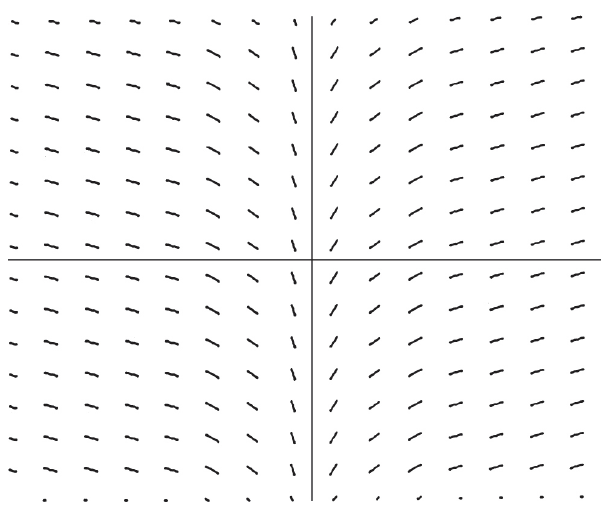
\includegraphics[width=0.6\linewidth]{data/calculus-figures/c11-a35.png}\end{center}
\begin{list}{}{\setlength{\leftmargin}{3em}\setlength{\labelwidth}{2.5em}\setlength{\itemsep}{0pt}\setlength{\topsep}{2pt}}
\item[(A)] quadratic
\item[(B)] cubic
\item[(C)] exponential
\item[(D)] logarithmic
\end{list}

\bigskip\noindent\textbf{A36.}\ $\lim_{h\to0}\dfrac1h\int_{\pi/4}^{\pi/4+h}\dfrac{\sin x}{x}\,dx=$
\begin{list}{}{\setlength{\leftmargin}{3em}\setlength{\labelwidth}{2.5em}\setlength{\itemsep}{0pt}\setlength{\topsep}{2pt}}
\item[(A)] $0$
\item[(B)] $1$
\item[(C)] $\sqrt2/2$
\item[(D)] $2\sqrt2/\pi$
\end{list}

\bigskip\noindent\textbf{A37.}\ The graph of $g$ consists of two quarter-circle arcs and two line segments. Find $\int_0^{12}g(x)\,dx$.
\begin{center}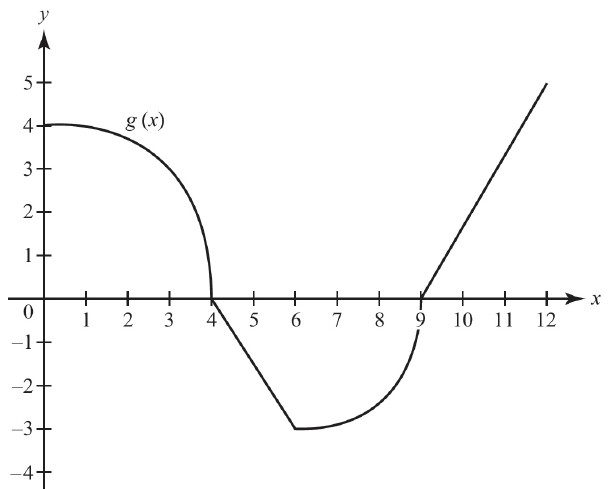
\includegraphics[width=0.6\linewidth]{data/calculus-figures/c11-a37.png}\end{center}
\begin{list}{}{\setlength{\leftmargin}{3em}\setlength{\labelwidth}{2.5em}\setlength{\itemsep}{0pt}\setlength{\topsep}{2pt}}
\item[(A)] $\pi+2$
\item[(B)] $7\pi/4+9/2$
\item[(C)] $7\pi/4+8$
\item[(D)] $25\pi/4+21/2$
\end{list}

\bigskip\noindent\textbf{A38.}\ Which could be a particular solution of the differential equation whose slope field is shown?
\begin{center}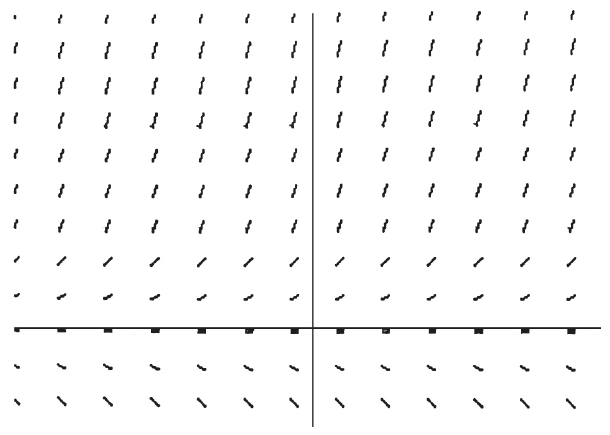
\includegraphics[width=0.6\linewidth]{data/calculus-figures/c11-a38.png}\end{center}
\begin{list}{}{\setlength{\leftmargin}{3em}\setlength{\labelwidth}{2.5em}\setlength{\itemsep}{0pt}\setlength{\topsep}{2pt}}
\item[(A)] $y=1/x$
\item[(B)] $y=\ln x$
\item[(C)] $y=e^x$
\item[(D)] $y=e^{-x}$
\end{list}

\bigskip\noindent\textbf{A39.}\ What is the domain of the particular solution $y=f(x)$ of $dy/dx=6x/(x^2-4)$ containing $(-1,\ln3)$?
\begin{list}{}{\setlength{\leftmargin}{3em}\setlength{\labelwidth}{2.5em}\setlength{\itemsep}{0pt}\setlength{\topsep}{2pt}}
\item[(A)] $x<0$
\item[(B)] $x>-2$
\item[(C)] $-2<x<2$
\item[(D)] $x\ne\pm2$
\end{list}

\bigskip\noindent\textbf{A40.}\ The slope field shown is for which differential equation?
\begin{center}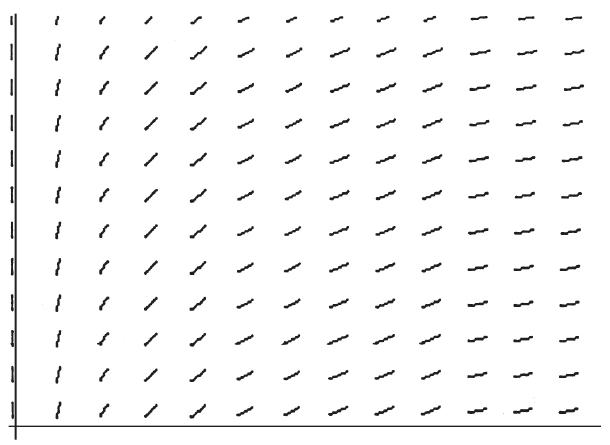
\includegraphics[width=0.6\linewidth]{data/calculus-figures/c11-a40.png}\end{center}
\begin{list}{}{\setlength{\leftmargin}{3em}\setlength{\labelwidth}{2.5em}\setlength{\itemsep}{0pt}\setlength{\topsep}{2pt}}
\item[(A)] $y^{\prime}=1/x$
\item[(B)] $y^{\prime}=\ln x$
\item[(C)] $y^{\prime}=e^x$
\item[(D)] $y^{\prime}=y^2$
\end{list}

\bigskip\noindent\textbf{A41.}\ With $x=\tan\theta$, which is equivalent to $\int_0^1\sqrt{1+x^2}\,dx$?
\begin{list}{}{\setlength{\leftmargin}{3em}\setlength{\labelwidth}{2.5em}\setlength{\itemsep}{0pt}\setlength{\topsep}{2pt}}
\item[(A)] $\int_0^1\sec\theta\,d\theta$
\item[(B)] $\int_0^{\pi/4}\sec\theta\,d\theta$
\item[(C)] $\int_0^{\pi/4}\sec^3\theta\,d\theta$
\item[(D)] $\int_0^{\tan1}\sec^3\theta\,d\theta$
\end{list}

\bigskip\noindent\textbf{A42.}\ If $x=2\sin u$ and $y=\cos2u$, a single equation in $x,y$ is
\begin{list}{}{\setlength{\leftmargin}{3em}\setlength{\labelwidth}{2.5em}\setlength{\itemsep}{0pt}\setlength{\topsep}{2pt}}
\item[(A)] $x^2+4y^2=4$
\item[(B)] $x^2+2y=2$
\item[(C)] $x^2+y^2=4$
\item[(D)] $x^2-2y=2$
\end{list}

\bigskip\noindent\textbf{A43.}\ Find the total area enclosed by the lemniscate $r^2=2\cos2\theta$.
\begin{list}{}{\setlength{\leftmargin}{3em}\setlength{\labelwidth}{2.5em}\setlength{\itemsep}{0pt}\setlength{\topsep}{2pt}}
\item[(A)] $4$
\item[(B)] $1$
\item[(C)] $1/4$
\item[(D)] $2$
\end{list}

\bigskip\noindent\textbf{A44.}\ $\int_{-\infty}^{\infty}\dfrac{dx}{x^2+1}=$
\begin{list}{}{\setlength{\leftmargin}{3em}\setlength{\labelwidth}{2.5em}\setlength{\itemsep}{0pt}\setlength{\topsep}{2pt}}
\item[(A)] $0$
\item[(B)] $\pi/2$
\item[(C)] $\pi$
\item[(D)] $2\pi$
\end{list}

\bigskip\noindent\textbf{A45.}\ The first four nonzero terms of the Maclaurin series for $f(x)=1/(1-2x)$ are
\begin{list}{}{\setlength{\leftmargin}{3em}\setlength{\labelwidth}{2.5em}\setlength{\itemsep}{0pt}\setlength{\topsep}{2pt}}
\item[(A)] $1+2x+4x^2+8x^3$
\item[(B)] $1-2x+4x^2-8x^3$
\item[(C)] $-1-2x-4x^2-8x^3$
\item[(D)] $1-x+x^2-x^3$
\end{list}

\bigskip\noindent\textbf{A46.}\ $\int x^2e^{-x}\,dx=$
\begin{list}{}{\setlength{\leftmargin}{3em}\setlength{\labelwidth}{2.5em}\setlength{\itemsep}{0pt}\setlength{\topsep}{2pt}}
\item[(A)] $-x^3e^{-x}/3+C$
\item[(B)] $-x^2e^{-x}+2xe^{-x}+C$
\item[(C)] $-x^2e^{-x}-2xe^{-x}-2e^{-x}+C$
\item[(D)] $-x^2e^{-x}+2xe^{-x}-2e^{-x}+C$
\end{list}

\bigskip\noindent\textbf{A47.}\ $\int_0^{\pi/2}\sin^2x\,dx=$
\begin{list}{}{\setlength{\leftmargin}{3em}\setlength{\labelwidth}{2.5em}\setlength{\itemsep}{0pt}\setlength{\topsep}{2pt}}
\item[(A)] $1/3$
\item[(B)] $\pi/4-1/4$
\item[(C)] $\pi/2$
\item[(D)] $\pi/4$
\end{list}

\bigskip\noindent\textbf{A48.}\ If $x=a\cot\theta$ and $y=a\sin^2\theta$, find $dy/dx$ at $\theta=\pi/4$.
\begin{list}{}{\setlength{\leftmargin}{3em}\setlength{\labelwidth}{2.5em}\setlength{\itemsep}{0pt}\setlength{\topsep}{2pt}}
\item[(A)] $1/2$
\item[(B)] $-2$
\item[(C)] $2$
\item[(D)] $-1/2$
\end{list}

\bigskip\noindent\textbf{A49.}\ Which improper integral diverges?
\begin{list}{}{\setlength{\leftmargin}{3em}\setlength{\labelwidth}{2.5em}\setlength{\itemsep}{0pt}\setlength{\topsep}{2pt}}
\item[(A)] $\int_{-\infty}^0e^x\,dx$
\item[(B)] $\int_0^1dx/x$
\item[(C)] $\int_0^\infty e^{-x}\,dx$
\item[(D)] $\int_0^1dx/\sqrt x$
\end{list}

\bigskip\noindent\textbf{A50.}\ $\int_2^4\dfrac{du}{\sqrt{16-u^2}}=$
\begin{list}{}{\setlength{\leftmargin}{3em}\setlength{\labelwidth}{2.5em}\setlength{\itemsep}{0pt}\setlength{\topsep}{2pt}}
\item[(A)] $\pi/12$
\item[(B)] $\pi/6$
\item[(C)] $\pi/3$
\item[(D)] $2\pi/3$
\end{list}

\bigskip\noindent\textbf{A51.}\ $\lim_{x\to0^+}(1/x)^x=$
\begin{list}{}{\setlength{\leftmargin}{3em}\setlength{\labelwidth}{2.5em}\setlength{\itemsep}{0pt}\setlength{\topsep}{2pt}}
\item[(A)] $0$
\item[(B)] $1$
\item[(C)] $\infty$
\item[(D)] nonexistent
\end{list}

\bigskip\noindent\textbf{A52.}\ A particle moves on $x=3y-y^2$ with $dy/dt=3$. Find its speed at $(2,1)$.
\begin{list}{}{\setlength{\leftmargin}{3em}\setlength{\labelwidth}{2.5em}\setlength{\itemsep}{0pt}\setlength{\topsep}{2pt}}
\item[(A)] $0$
\item[(B)] $3$
\item[(C)] $3\sqrt2$
\item[(D)] $\sqrt{13}$
\end{list}

\bigskip\noindent\textbf{A53.}\ $\lim_{x\to0^+}\dfrac{\cot x}{\ln x}=$
\begin{list}{}{\setlength{\leftmargin}{3em}\setlength{\labelwidth}{2.5em}\setlength{\itemsep}{0pt}\setlength{\topsep}{2pt}}
\item[(A)] $-\infty$
\item[(B)] $-1$
\item[(C)] $0$
\item[(D)] $1$
\end{list}

\bigskip\noindent\textbf{A54.}\ Which terms occur in the partial fraction decomposition of $(3x+2)/(x^2-x-12)$? I. $1/(x+3)$; II. $1/(x-4)$; III. $2/(x-4)$.
\begin{list}{}{\setlength{\leftmargin}{3em}\setlength{\labelwidth}{2.5em}\setlength{\itemsep}{0pt}\setlength{\topsep}{2pt}}
\item[(A)] none
\item[(B)] I only
\item[(C)] II only
\item[(D)] I and III only
\end{list}

\bigskip\noindent\textbf{A55.}\ Using three terms of an appropriate Maclaurin series, estimate $\int_0^1(1-\cos x)/x\,dx$.
\begin{list}{}{\setlength{\leftmargin}{3em}\setlength{\labelwidth}{2.5em}\setlength{\itemsep}{0pt}\setlength{\topsep}{2pt}}
\item[(A)] $1/96$
\item[(B)] $23/96$
\item[(C)] $25/96$
\item[(D)] undefined; the integral is improper
\end{list}

\bigskip\noindent\textbf{A56.}\ Find the slope of the spiral $r=\theta$ at $\theta=\pi/4$.
\begin{list}{}{\setlength{\leftmargin}{3em}\setlength{\labelwidth}{2.5em}\setlength{\itemsep}{0pt}\setlength{\topsep}{2pt}}
\item[(A)] $-\sqrt2$
\item[(B)] $-1$
\item[(C)] $1$
\item[(D)] $(4+\pi)/(4-\pi)$
\end{list}

\bigskip\noindent\textbf{A57.}\ $\int_0^{\pi/3}\sec^2x\tan^2x\,dx=$
\begin{list}{}{\setlength{\leftmargin}{3em}\setlength{\labelwidth}{2.5em}\setlength{\itemsep}{0pt}\setlength{\topsep}{2pt}}
\item[(A)] $\sqrt3/27$
\item[(B)] $\sqrt3/3$
\item[(C)] $\sqrt3$
\item[(D)] $3\sqrt3$
\end{list}

\bigskip\noindent\textbf{A58.}\ A particle has acceleration $a=6t$ and $v(0)=1$. Find the total distance traveled from $t=0$ to $t=3$.
\begin{list}{}{\setlength{\leftmargin}{3em}\setlength{\labelwidth}{2.5em}\setlength{\itemsep}{0pt}\setlength{\topsep}{2pt}}
\item[(A)] $30$
\item[(B)] $28$
\item[(C)] $27$
\item[(D)] $26$
\end{list}

\bigskip\noindent\textbf{A59.}\ Air escapes from a balloon at $R(t)=60/(1+t^2)$ cubic feet per minute. How many cubic feet escape during the first minute?
\begin{list}{}{\setlength{\leftmargin}{3em}\setlength{\labelwidth}{2.5em}\setlength{\itemsep}{0pt}\setlength{\topsep}{2pt}}
\item[(A)] $15\pi$
\item[(B)] $30$
\item[(C)] $45$
\item[(D)] $30\ln2$
\end{list}

\bigskip\noindent\textbf{B1.}\ The graph of $h$ is shown. Which statements are true? I. $h^{\prime}$ is never negative. II. $h^{\prime\prime}$ is constant. III. $h^{\prime}$ and $h^{\prime\prime}$ equal zero at the same point.
\begin{center}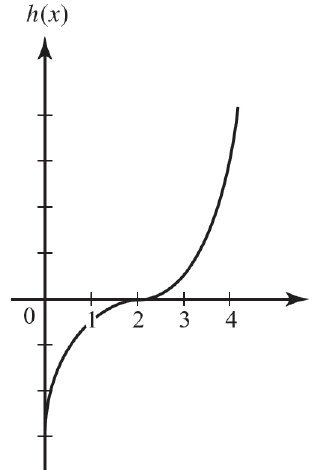
\includegraphics[width=0.6\linewidth]{data/calculus-figures/c11-b1.png}\end{center}
\begin{list}{}{\setlength{\leftmargin}{3em}\setlength{\labelwidth}{2.5em}\setlength{\itemsep}{0pt}\setlength{\topsep}{2pt}}
\item[(A)] I only
\item[(B)] III only
\item[(C)] I and II only
\item[(D)] I and III only
\end{list}

\bigskip\noindent\textbf{B2.}\ For the shown graphs, which statements are true? I. $g=f^{\prime}$. II. $f=g^{\prime}$. III. $h=g^{\prime\prime}$.
\begin{center}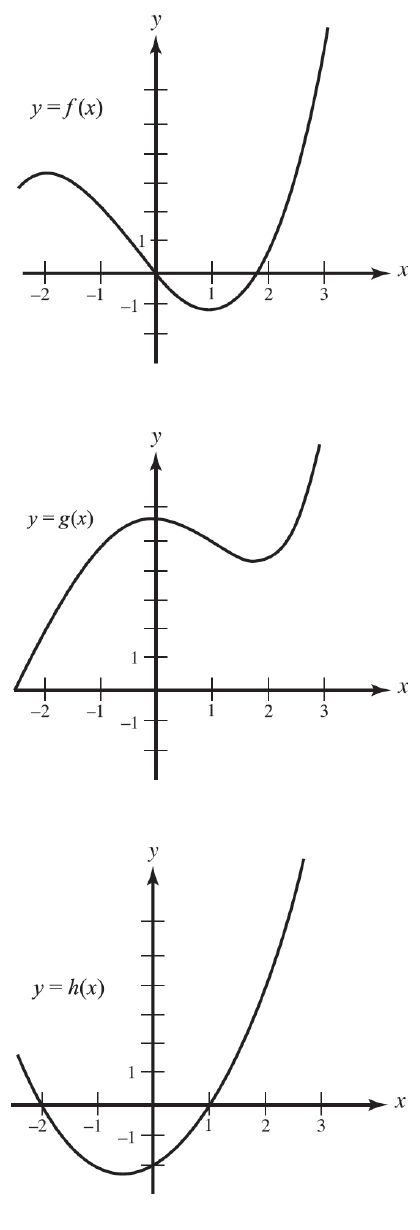
\includegraphics[width=0.6\linewidth]{data/calculus-figures/c11-b2.png}\end{center}
\begin{list}{}{\setlength{\leftmargin}{3em}\setlength{\labelwidth}{2.5em}\setlength{\itemsep}{0pt}\setlength{\topsep}{2pt}}
\item[(A)] I only
\item[(B)] II only
\item[(C)] II and III only
\item[(D)] I, II, and III
\end{list}

\bigskip\noindent\textbf{B3.}\ If $y=\int_3^x(3+2t)^{-1/2}\,dt$, find $d^2y/dx^2$.
\begin{list}{}{\setlength{\leftmargin}{3em}\setlength{\labelwidth}{2.5em}\setlength{\itemsep}{0pt}\setlength{\topsep}{2pt}}
\item[(A)] $-1/(3+2x)^{3/2}$
\item[(B)] $3/(3+2x)^{5/2}$
\item[(C)] $\sqrt{3+2x}/2$
\item[(D)] $(3+2x)^{3/2}/3$
\end{list}

\bigskip\noindent\textbf{B4.}\ If $\int_{-3}^4 f(x)\,dx=6$, find $\int_{-4}^3 f(x+1)\,dx$.
\begin{list}{}{\setlength{\leftmargin}{3em}\setlength{\labelwidth}{2.5em}\setlength{\itemsep}{0pt}\setlength{\topsep}{2pt}}
\item[(A)] $-6$
\item[(B)] $-5$
\item[(C)] $5$
\item[(D)] $6$
\end{list}

\bigskip\noindent\textbf{B5.}\ At what point of $[1,1.5]$ does the instantaneous rate of change of $f(x)=\sin x$ equal its average rate on this interval?
\begin{list}{}{\setlength{\leftmargin}{3em}\setlength{\labelwidth}{2.5em}\setlength{\itemsep}{0pt}\setlength{\topsep}{2pt}}
\item[(A)] $1.058$
\item[(B)] $1.239$
\item[(C)] $1.253$
\item[(D)] $1.399$
\end{list}

\bigskip\noindent\textbf{B6.}\ Let $f^{\prime}(x)=x^2(x-1)$, so $f^{\prime\prime}(x)=x(3x-2)$. On which intervals is $f$ increasing and concave up? I. $x<0$; II. $0<x<2/3$; III. $2/3<x<1$; IV. $x>1$.
\begin{list}{}{\setlength{\leftmargin}{3em}\setlength{\labelwidth}{2.5em}\setlength{\itemsep}{0pt}\setlength{\topsep}{2pt}}
\item[(A)] I only
\item[(B)] II and IV only
\item[(C)] I and III only
\item[(D)] IV only
\end{list}

\bigskip\noindent\textbf{B7.}\ Let $f^{\prime}(x)=x^2(x-1)$ and $f^{\prime\prime}(x)=x(3x-2)$. Which statement is true?
\begin{list}{}{\setlength{\leftmargin}{3em}\setlength{\labelwidth}{2.5em}\setlength{\itemsep}{0pt}\setlength{\topsep}{2pt}}
\item[(A)] One relative extremum and one inflection point.
\item[(B)] One relative extremum and two inflection points.
\item[(C)] Two relative extrema and one inflection point.
\item[(D)] Two relative extrema and two inflection points.
\end{list}

\bigskip\noindent\textbf{B8.}\ The $n$th derivative of $\ln(x+1)$ at $x=2$, for $n\ge1$, equals
\begin{list}{}{\setlength{\leftmargin}{3em}\setlength{\labelwidth}{2.5em}\setlength{\itemsep}{0pt}\setlength{\topsep}{2pt}}
\item[(A)] $(-1)^n n!/3^{n+1}$
\item[(B)] $(-1)^{n-1}(n-1)!/3^n$
\item[(C)] $(-1)^{n+1}n!/3^{n+1}$
\item[(D)] $(-1)^{n+1}/3^{n+1}$
\end{list}

\bigskip\noindent\textbf{B9.}\ If $f$ is continuous at $x=a$, which statement may be false?
\begin{list}{}{\setlength{\leftmargin}{3em}\setlength{\labelwidth}{2.5em}\setlength{\itemsep}{0pt}\setlength{\topsep}{2pt}}
\item[(A)] $\lim_{x\to a}f(x)=f(a)$
\item[(B)] $f^{\prime}(a)$ exists
\item[(C)] $f(a)$ is defined
\item[(D)] $\lim_{x\to a^-}f(x)=\lim_{x\to a^+}f(x)$
\end{list}

\bigskip\noindent\textbf{B10.}\ If $\int_0^3 f(x+k)\,dx=4$ for constant $k$, find $\int_k^{3+k}f(x)\,dx$.
\begin{list}{}{\setlength{\leftmargin}{3em}\setlength{\labelwidth}{2.5em}\setlength{\itemsep}{0pt}\setlength{\topsep}{2pt}}
\item[(A)] $3$
\item[(B)] $4-k$
\item[(C)] $4$
\item[(D)] $4+k$
\end{list}

\bigskip\noindent\textbf{B11.}\ Find the volume in cubic feet of an inner tube with inner diameter 4 feet and outer diameter 8 feet.
\begin{list}{}{\setlength{\leftmargin}{3em}\setlength{\labelwidth}{2.5em}\setlength{\itemsep}{0pt}\setlength{\topsep}{2pt}}
\item[(A)] $6\pi^2$
\item[(B)] $12\pi^2$
\item[(C)] $24\pi^2$
\item[(D)] $48\pi^2$
\end{list}

\bigskip\noindent\textbf{B12.}\ If $f(u)=\arctan(u^2)$ and $g(u)=e^u$, find the derivative of $f(g(u))$.
\begin{list}{}{\setlength{\leftmargin}{3em}\setlength{\labelwidth}{2.5em}\setlength{\itemsep}{0pt}\setlength{\topsep}{2pt}}
\item[(A)] $2ue^u/(1+u^4)$
\item[(B)] $2ue^{u^2}/(1+u^4)$
\item[(C)] $2e^u/(1+4e^{2u})$
\item[(D)] $2e^{2u}/(1+e^{4u})$
\end{list}

\bigskip\noindent\textbf{B13.}\ If $\sin(xy)=y$, find $dy/dx$.
\begin{list}{}{\setlength{\leftmargin}{3em}\setlength{\labelwidth}{2.5em}\setlength{\itemsep}{0pt}\setlength{\topsep}{2pt}}
\item[(A)] $y\cos(xy)-1$
\item[(B)] $(1-y\cos(xy))/(x\cos(xy))$
\item[(C)] $y\cos(xy)/(1-x\cos(xy))$
\item[(D)] $\cos(xy)$
\end{list}

\bigskip\noindent\textbf{B14.}\ For $x>0$, suppose $f^{\prime}(x)=g(x)$ and $g^{\prime}(x)=f(\sqrt x)$. Find $\dfrac{d^2}{dx^2}f(x^2)$.
\begin{list}{}{\setlength{\leftmargin}{3em}\setlength{\labelwidth}{2.5em}\setlength{\itemsep}{0pt}\setlength{\topsep}{2pt}}
\item[(A)] $f(x^2)$
\item[(B)] $2xg(x^2)$
\item[(C)] $f(x)/(2x)$
\item[(D)] $2g(x^2)+4x^2f(x)$
\end{list}

\bigskip\noindent\textbf{B15.}\ The region bounded by $y=e^x$, $y=1$, and $x=2$ is rotated about the $x$-axis. Which integral gives its volume?
\begin{list}{}{\setlength{\leftmargin}{3em}\setlength{\labelwidth}{2.5em}\setlength{\itemsep}{0pt}\setlength{\topsep}{2pt}}
\item[(A)] $\pi\int_0^2e^{2x}dx$
\item[(B)] $2\pi\int_1^{e^2}(2-\ln y)(y-1)dy$
\item[(C)] $\pi\int_0^2(e^{2x}-1)dx$
\item[(D)] $\pi\int_0^2(e^x-1)^2dx$
\end{list}

\bigskip\noindent\textbf{B16.}\ Suppose $f$ is continuous on $[1,2]$, differentiable on $(1,2)$, $f(1)=3$, and $f(2)=0$. Which is not necessarily true?
\begin{list}{}{\setlength{\leftmargin}{3em}\setlength{\labelwidth}{2.5em}\setlength{\itemsep}{0pt}\setlength{\topsep}{2pt}}
\item[(A)] $\int_1^2f(x)dx$ exists.
\item[(B)] Some $c\in(1,2)$ has $f^{\prime}(c)=0$.
\item[(C)] Every value between 0 and 3 is attained between 1 and 2.
\item[(D)] $\lim_{x\to c}f(x)$ exists for every $1<c<2$.
\end{list}

\bigskip\noindent\textbf{B17.}\ The region $S$ bounded by $y=\sec x$, the $y$-axis, and $y=4$ is rotated about the $y$-axis. Find the volume.
\begin{center}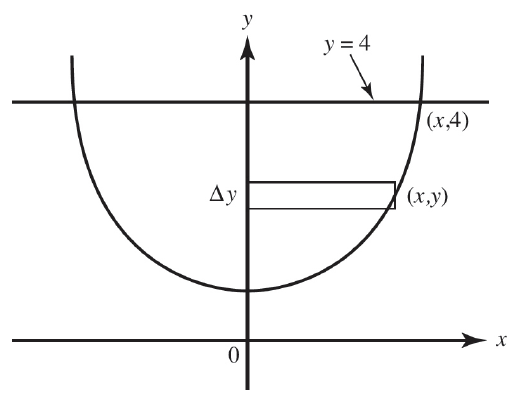
\includegraphics[width=0.6\linewidth]{data/calculus-figures/c11-b17.png}\end{center}
\begin{list}{}{\setlength{\leftmargin}{3em}\setlength{\labelwidth}{2.5em}\setlength{\itemsep}{0pt}\setlength{\topsep}{2pt}}
\item[(A)] $2.279$
\item[(B)] $5.692$
\item[(C)] $11.385$
\item[(D)] $17.217$
\end{list}

\bigskip\noindent\textbf{B18.}\ A radioactive substance decreases from 40 grams to 20 grams in two years. To the nearest gram, how much remains after three years?
\begin{list}{}{\setlength{\leftmargin}{3em}\setlength{\labelwidth}{2.5em}\setlength{\itemsep}{0pt}\setlength{\topsep}{2pt}}
\item[(A)] $10$
\item[(B)] $12$
\item[(C)] $14$
\item[(D)] $16$
\end{list}

\bigskip\noindent\textbf{B19.}\ An object moving on a line has $a(t)=\pi t+2/(1+t^2)$ and is at rest at $t=1$. Find its average velocity from $t=0$ to $t=2$.
\begin{list}{}{\setlength{\leftmargin}{3em}\setlength{\labelwidth}{2.5em}\setlength{\itemsep}{0pt}\setlength{\topsep}{2pt}}
\item[(A)] $0.362$
\item[(B)] $0.274$
\item[(C)] $3.504$
\item[(D)] $4.249$
\end{list}

\bigskip\noindent\textbf{B20.}\ Find the area bounded by $y=\tan x$, $x+y=2$, and the $x$-axis on $[0,2]$.
\begin{list}{}{\setlength{\leftmargin}{3em}\setlength{\labelwidth}{2.5em}\setlength{\itemsep}{0pt}\setlength{\topsep}{2pt}}
\item[(A)] $0.919$
\item[(B)] $1.013$
\item[(C)] $1.077$
\item[(D)] $1.494$
\end{list}

\bigskip\noindent\textbf{B21.}\ An ellipse has major axis 20 and minor axis 10. Find the maximum area of an inscribed rectangle, rounded to the nearest integer.
\begin{list}{}{\setlength{\leftmargin}{3em}\setlength{\labelwidth}{2.5em}\setlength{\itemsep}{0pt}\setlength{\topsep}{2pt}}
\item[(A)] $50$
\item[(B)] $79$
\item[(C)] $82$
\item[(D)] $100$
\end{list}

\bigskip\noindent\textbf{B22.}\ Find the average value of $y=x\ln x$ on $[1,e]$.
\begin{list}{}{\setlength{\leftmargin}{3em}\setlength{\labelwidth}{2.5em}\setlength{\itemsep}{0pt}\setlength{\topsep}{2pt}}
\item[(A)] $0.772$
\item[(B)] $1.221$
\item[(C)] $1.359$
\item[(D)] $2.097$
\end{list}

\bigskip\noindent\textbf{B23.}\ Let $f(x)=\int_0^x(1-2\cos^3t)dt$ for $0\le x\le2\pi$. On which interval is $f$ increasing?
\begin{list}{}{\setlength{\leftmargin}{3em}\setlength{\labelwidth}{2.5em}\setlength{\itemsep}{0pt}\setlength{\topsep}{2pt}}
\item[(A)] $0<x<\pi$
\item[(B)] $0.654<x<5.629$
\item[(C)] $0.654<x<2\pi$
\item[(D)] $\pi<x<2\pi$
\end{list}

\bigskip\noindent\textbf{B24.}\ The table gives speed in ft/sec: $\begin{array}{c|rrrr}t\ (\mathrm{sec})&0&1&3&6\\ \text{speed}&30&22&12&6\end{array}$. Estimate acceleration at $t=2$ in ft/sec$^2$.
\begin{list}{}{\setlength{\leftmargin}{3em}\setlength{\labelwidth}{2.5em}\setlength{\itemsep}{0pt}\setlength{\topsep}{2pt}}
\item[(A)] $-10$
\item[(B)] $-6$
\item[(C)] $-5$
\item[(D)] $-10/3$
\end{list}

\bigskip\noindent\textbf{B25.}\ A 16-foot-high syrup tank has back $y=x^2$ and square horizontal cross sections. Syrup enters at $12$ ft$^3$/hr. How fast is its depth rising when it is 9 feet deep?
\begin{center}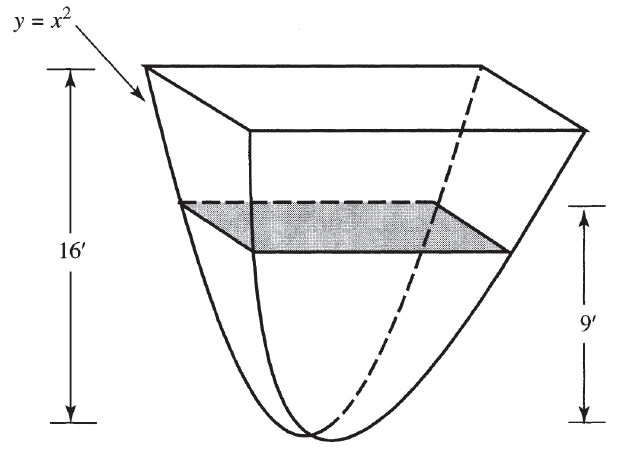
\includegraphics[width=0.6\linewidth]{data/calculus-figures/c11-b25.png}\end{center}
\begin{list}{}{\setlength{\leftmargin}{3em}\setlength{\labelwidth}{2.5em}\setlength{\itemsep}{0pt}\setlength{\topsep}{2pt}}
\item[(A)] $2/27$
\item[(B)] $1/3$
\item[(C)] $4/3$
\item[(D)] $36$
\end{list}

\bigskip\noindent\textbf{B26.}\ A deer population satisfies $dP/dt=k(1000-P)$. Initially $P(0)=300$, and $P(5)=500$. How many deer will there be after 10 years?
\begin{list}{}{\setlength{\leftmargin}{3em}\setlength{\labelwidth}{2.5em}\setlength{\itemsep}{0pt}\setlength{\topsep}{2pt}}
\item[(A)] $608$
\item[(B)] $643$
\item[(C)] $700$
\item[(D)] $833$
\end{list}

\bigskip\noindent\textbf{B27.}\ The graph shows $f(x)=4/(x^2+1)$. Let $H(x)=\int_0^xf(t)dt$. Find the local linearization of $H$ at $x=1$.
\begin{center}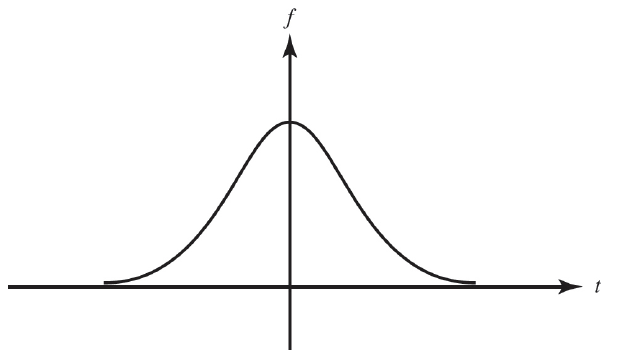
\includegraphics[width=0.6\linewidth]{data/calculus-figures/c11-b27.png}\end{center}
\begin{list}{}{\setlength{\leftmargin}{3em}\setlength{\labelwidth}{2.5em}\setlength{\itemsep}{0pt}\setlength{\topsep}{2pt}}
\item[(A)] $y=2x$
\item[(B)] $y=-2x-4$
\item[(C)] $y=2x+\pi-2$
\item[(D)] $y=-2x+\pi+2$
\end{list}

\bigskip\noindent\textbf{B28.}\ A 100-foot smokestack has diameters (feet) at these heights (feet): $\begin{array}{c|rrrrr}h&0&10&50&70&100\\d&17&15&9&7&5\end{array}$. Use a left Riemann sum on the four indicated intervals to estimate volume to the nearest cubic foot.
\begin{list}{}{\setlength{\leftmargin}{3em}\setlength{\labelwidth}{2.5em}\setlength{\itemsep}{0pt}\setlength{\topsep}{2pt}}
\item[(A)] $1160$
\item[(B)] $5671$
\item[(C)] $8718$
\item[(D)] $11765$
\end{list}

\bigskip\noindent\textbf{B29.}\ Differentiable functions $f,g$ have values $\begin{array}{c|rrrr}x&f(x)&f^{\prime}(x)&g(x)&g^{\prime}(x)\\1&2&1/2&-3&5\\2&3&1&0&4\\3&4&2&2&3\\4&6&4&3&1/2\end{array}$. If $P(x)=f(x)/g(x)$, find $P^{\prime}(3)$.
\begin{list}{}{\setlength{\leftmargin}{3em}\setlength{\labelwidth}{2.5em}\setlength{\itemsep}{0pt}\setlength{\topsep}{2pt}}
\item[(A)] $-2$
\item[(B)] $-8/9$
\item[(C)] $2/3$
\item[(D)] $2$
\end{list}

\bigskip\noindent\textbf{B30.}\ Differentiable functions $f,g$ have values $\begin{array}{c|rrrr}x&f(x)&f^{\prime}(x)&g(x)&g^{\prime}(x)\\1&2&1/2&-3&5\\2&3&1&0&4\\3&4&2&2&3\\4&6&4&3&1/2\end{array}$. If $H(x)=f(g(x))$, find $H^{\prime}(3)$.
\begin{list}{}{\setlength{\leftmargin}{3em}\setlength{\labelwidth}{2.5em}\setlength{\itemsep}{0pt}\setlength{\topsep}{2pt}}
\item[(A)] $1$
\item[(B)] $2$
\item[(C)] $3$
\item[(D)] $6$
\end{list}

\bigskip\noindent\textbf{B31.}\ Differentiable functions $f,g$ have values $\begin{array}{c|rrrr}x&f(x)&f^{\prime}(x)&g(x)&g^{\prime}(x)\\1&2&1/2&-3&5\\2&3&1&0&4\\3&4&2&2&3\\4&6&4&3&1/2\end{array}$. If $M(x)=f(x)g(x)$, find $M^{\prime}(3)$.
\begin{list}{}{\setlength{\leftmargin}{3em}\setlength{\labelwidth}{2.5em}\setlength{\itemsep}{0pt}\setlength{\topsep}{2pt}}
\item[(A)] $2$
\item[(B)] $6$
\item[(C)] $8$
\item[(D)] $16$
\end{list}

\bigskip\noindent\textbf{B32.}\ Differentiable functions $f,g$ have values $\begin{array}{c|rrrr}x&f(x)&f^{\prime}(x)&g(x)&g^{\prime}(x)\\1&2&1/2&-3&5\\2&3&1&0&4\\3&4&2&2&3\\4&6&4&3&1/2\end{array}$. If $K(x)=g^{-1}(x)$, find $K^{\prime}(3)$.
\begin{list}{}{\setlength{\leftmargin}{3em}\setlength{\labelwidth}{2.5em}\setlength{\itemsep}{0pt}\setlength{\topsep}{2pt}}
\item[(A)] $-1/3$
\item[(B)] $1/3$
\item[(C)] $1/2$
\item[(D)] $2$
\end{list}

\bigskip\noindent\textbf{B33.}\ Differentiable functions $f,g$ have values $\begin{array}{c|rrrr}x&f(x)&f^{\prime}(x)&g(x)&g^{\prime}(x)\\1&2&1/2&-3&5\\2&3&1&0&4\\3&4&2&2&3\\4&6&4&3&1/2\end{array}$. If $R(x)=\sqrt{f(x)}$, find $R^{\prime}(3)$.
\begin{list}{}{\setlength{\leftmargin}{3em}\setlength{\labelwidth}{2.5em}\setlength{\itemsep}{0pt}\setlength{\topsep}{2pt}}
\item[(A)] $1/4$
\item[(B)] $1/(2\sqrt2)$
\item[(C)] $1/2$
\item[(D)] $\sqrt2$
\end{list}

\bigskip\noindent\textbf{B34.}\ Water enters a spherical tank at a constant rate. If $W(t)$ is the rate of increase of water depth, then $W$ is
\begin{list}{}{\setlength{\leftmargin}{3em}\setlength{\labelwidth}{2.5em}\setlength{\itemsep}{0pt}\setlength{\topsep}{2pt}}
\item[(A)] linear and increasing
\item[(B)] linear and decreasing
\item[(C)] concave up
\item[(D)] concave down
\end{list}

\bigskip\noindent\textbf{B35.}\ The graph of $f^{\prime}$ is shown. If $f(7)=3$, find $f(1)$.
\begin{center}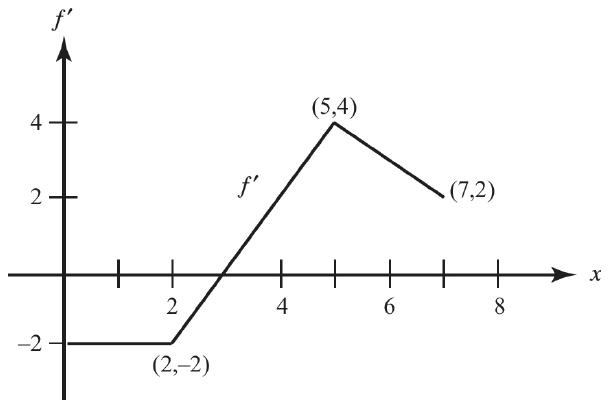
\includegraphics[width=0.6\linewidth]{data/calculus-figures/c11-b35.png}\end{center}
\begin{list}{}{\setlength{\leftmargin}{3em}\setlength{\labelwidth}{2.5em}\setlength{\itemsep}{0pt}\setlength{\topsep}{2pt}}
\item[(A)] $-10$
\item[(B)] $-4$
\item[(C)] $10$
\item[(D)] $16$
\end{list}

\bigskip\noindent\textbf{B36.}\ A concert crowd fills a semicircular disk of radius 100 yards centered at the stage. Its density $x$ yards from the stage is $D(x)=20/(2\sqrt x+1)$ people per square yard. About how many people attend?
\begin{center}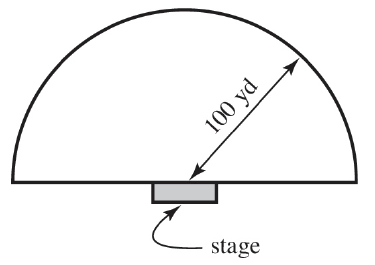
\includegraphics[width=0.6\linewidth]{data/calculus-figures/c11-b36.png}\end{center}
\begin{list}{}{\setlength{\leftmargin}{3em}\setlength{\labelwidth}{2.5em}\setlength{\itemsep}{0pt}\setlength{\topsep}{2pt}}
\item[(A)] $200$
\item[(B)] $19500$
\item[(C)] $21000$
\item[(D)] $165000$
\end{list}

\bigskip\noindent\textbf{B37.}\ More AIDS cases were reported this year, but the rate of increase is slowing. As a function of time, the number of cases is currently
\begin{list}{}{\setlength{\leftmargin}{3em}\setlength{\labelwidth}{2.5em}\setlength{\itemsep}{0pt}\setlength{\topsep}{2pt}}
\item[(A)] increasing and concave down
\item[(B)] increasing and concave up
\item[(C)] decreasing and concave down
\item[(D)] decreasing and concave up
\end{list}

\bigskip\noindent\textbf{B38.}\ The graph shows velocity in ft/sec over $0\le t\le8$ for an object moving along a line. Find its average speed on this interval.
\begin{center}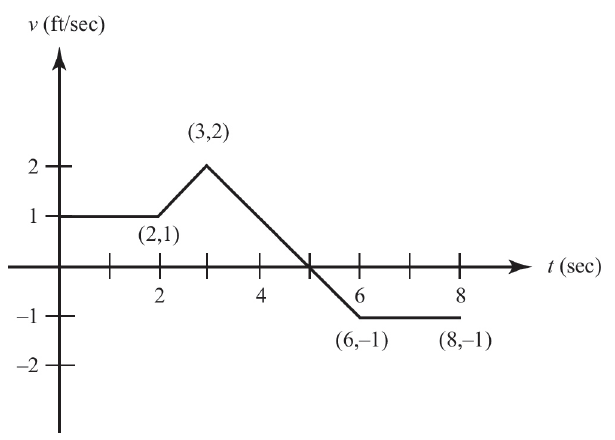
\includegraphics[width=0.6\linewidth]{data/calculus-figures/c11-b38-40.png}\end{center}
\begin{list}{}{\setlength{\leftmargin}{3em}\setlength{\labelwidth}{2.5em}\setlength{\itemsep}{0pt}\setlength{\topsep}{2pt}}
\item[(A)] $3/8$
\item[(B)] $1$
\item[(C)] $8/3$
\item[(D)] $8$
\end{list}

\bigskip\noindent\textbf{B39.}\ The graph shows velocity in ft/sec over $0\le t\le8$ for an object moving along a line. When did the object return to its position at $t=2$?
\begin{center}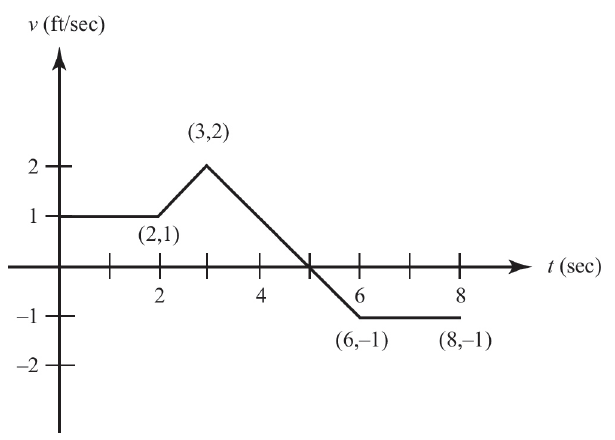
\includegraphics[width=0.6\linewidth]{data/calculus-figures/c11-b38-40.png}\end{center}
\begin{list}{}{\setlength{\leftmargin}{3em}\setlength{\labelwidth}{2.5em}\setlength{\itemsep}{0pt}\setlength{\topsep}{2pt}}
\item[(A)] $t=6$
\item[(B)] $t=7$
\item[(C)] $t=8$
\item[(D)] never
\end{list}

\bigskip\noindent\textbf{B40.}\ The graph shows velocity in ft/sec over $0\le t\le8$ for an object moving along a line. Find its average acceleration in ft/sec$^2$.
\begin{center}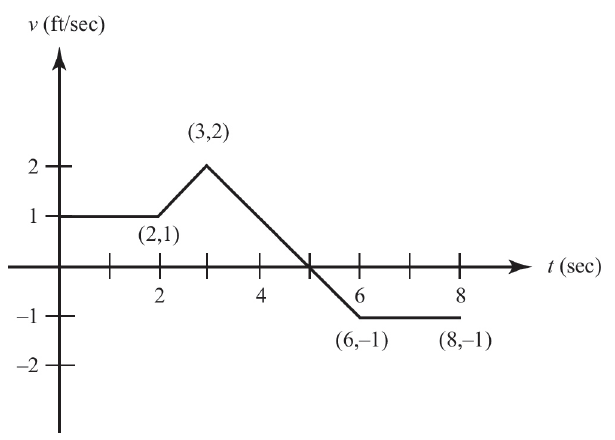
\includegraphics[width=0.6\linewidth]{data/calculus-figures/c11-b38-40.png}\end{center}
\begin{list}{}{\setlength{\leftmargin}{3em}\setlength{\labelwidth}{2.5em}\setlength{\itemsep}{0pt}\setlength{\topsep}{2pt}}
\item[(A)] $-2$
\item[(B)] $-1/4$
\item[(C)] $1/4$
\item[(D)] $1$
\end{list}

\bigskip\noindent\textbf{B41.}\ Ice melts at $M(t)=72/(2t+3)$ cm$^3$/min. Approximately how much melts in the first three minutes?
\begin{list}{}{\setlength{\leftmargin}{3em}\setlength{\labelwidth}{2.5em}\setlength{\itemsep}{0pt}\setlength{\topsep}{2pt}}
\item[(A)] $8$ cm$^3$
\item[(B)] $16$ cm$^3$
\item[(C)] $21$ cm$^3$
\item[(D)] $40$ cm$^3$
\end{list}

\bigskip\noindent\textbf{B42.}\ A particle moves counterclockwise on $x^2+y^2=25$ with speed 2 ft/sec. Find its velocity vector at $(3,4)$.
\begin{list}{}{\setlength{\leftmargin}{3em}\setlength{\labelwidth}{2.5em}\setlength{\itemsep}{0pt}\setlength{\topsep}{2pt}}
\item[(A)] $\langle-8/5,6/5\rangle$
\item[(B)] $\langle8/5,-6/5\rangle$
\item[(C)] $\langle-2\sqrt3,2\rangle$
\item[(D)] $\langle2,-2\sqrt3\rangle$
\end{list}

\bigskip\noindent\textbf{B43.}\ Let $\mathbf R(t)=\langle a\cos kt,a\sin kt\rangle$ with $a,k>0$. Find the acceleration vector.
\begin{list}{}{\setlength{\leftmargin}{3em}\setlength{\labelwidth}{2.5em}\setlength{\itemsep}{0pt}\setlength{\topsep}{2pt}}
\item[(A)] $-k^2\mathbf R$
\item[(B)] $a^2k^2\mathbf R$
\item[(C)] $-a\mathbf R$
\item[(D)] $-ak^2\langle a\cos kt,a\sin kt\rangle$
\end{list}

\bigskip\noindent\textbf{B44.}\ Find the length of $y=2^x$ between $(0,1)$ and $(2,4)$.
\begin{list}{}{\setlength{\leftmargin}{3em}\setlength{\labelwidth}{2.5em}\setlength{\itemsep}{0pt}\setlength{\topsep}{2pt}}
\item[(A)] $3.141$
\item[(B)] $3.664$
\item[(C)] $4.823$
\item[(D)] $7.199$
\end{list}

\bigskip\noindent\textbf{B45.}\ A moving object has position $P(t)=(3t,e^t)$. Its acceleration is
\begin{list}{}{\setlength{\leftmargin}{3em}\setlength{\labelwidth}{2.5em}\setlength{\itemsep}{0pt}\setlength{\topsep}{2pt}}
\item[(A)] constant in both magnitude and direction
\item[(B)] constant in magnitude only
\item[(C)] constant in direction only
\item[(D)] constant in neither magnitude nor direction
\end{list}

\bigskip\noindent\textbf{B46.}\ Apply one Euler step of size $\Delta x=0.1$ to $dy/dx=4y$ starting at $(0,1)$. Approximately how large is the error?
\begin{list}{}{\setlength{\leftmargin}{3em}\setlength{\labelwidth}{2.5em}\setlength{\itemsep}{0pt}\setlength{\topsep}{2pt}}
\item[(A)] $0.09$
\item[(B)] $1.09$
\item[(C)] $1.49$
\item[(D)] $1.90$
\end{list}

\bigskip\noindent\textbf{B47.}\ Use the first three terms to estimate $\sum_{n=0}^{\infty}(-1)^n/(n^2+1)$. Which statements are true? I. The estimate is 0.7. II. It is too low. III. The error is less than 0.1.
\begin{list}{}{\setlength{\leftmargin}{3em}\setlength{\labelwidth}{2.5em}\setlength{\itemsep}{0pt}\setlength{\topsep}{2pt}}
\item[(A)] I only
\item[(B)] III only
\item[(C)] I and III only
\item[(D)] I, II, and III
\end{list}

\bigskip\noindent\textbf{B48.}\ Which series diverges?
\begin{list}{}{\setlength{\leftmargin}{3em}\setlength{\labelwidth}{2.5em}\setlength{\itemsep}{0pt}\setlength{\topsep}{2pt}}
\item[(A)] $\sum_{n=1}^{\infty}2/3^n$
\item[(B)] $\sum_{n=1}^{\infty}2/(3n)$
\item[(C)] $\sum_{n=1}^{\infty}2/n^3$
\item[(D)] $\sum_{n=1}^{\infty}2n/3^n$
\end{list}

\bigskip\noindent\textbf{B49.}\ Find the radius of convergence of $\sum_{n=1}^{\infty}(n!/n^n)x^n$.
\begin{list}{}{\setlength{\leftmargin}{3em}\setlength{\labelwidth}{2.5em}\setlength{\itemsep}{0pt}\setlength{\topsep}{2pt}}
\item[(A)] $0$
\item[(B)] $1/e$
\item[(C)] $1$
\item[(D)] $e$
\end{list}

\bigskip\noindent\textbf{B50.}\ Using $e^x\approx1+x+x^2/2$ to estimate $\sqrt e$, apply the Lagrange remainder bound with $M=\max_{0\le t\le1/2}e^t$. Which is the smallest listed upper bound supplied by this estimate?
\begin{list}{}{\setlength{\leftmargin}{3em}\setlength{\labelwidth}{2.5em}\setlength{\itemsep}{0pt}\setlength{\topsep}{2pt}}
\item[(A)] $0.021$
\item[(B)] $0.035$
\item[(C)] $0.057$
\item[(D)] $0.063$
\end{list}

\bigskip\noindent\textbf{B51.}\ An object has position $P(t)=(\tan t,\cos2t)$ for $0\le t\le1$. How far does it travel?
\begin{list}{}{\setlength{\leftmargin}{3em}\setlength{\labelwidth}{2.5em}\setlength{\itemsep}{0pt}\setlength{\topsep}{2pt}}
\item[(A)] $0.952$
\item[(B)] $1.726$
\item[(C)] $1.910$
\item[(D)] $2.140$
\end{list}

\bigskip\noindent\textbf{B52.}\ The region $S$ shown is bounded by $y=\sec x$ and $y=4$. Find the volume when it is rotated about the $x$-axis.
\begin{center}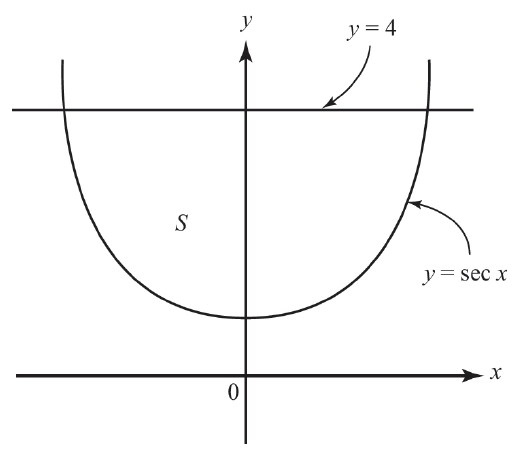
\includegraphics[width=0.6\linewidth]{data/calculus-figures/c11-b52.png}\end{center}
\begin{list}{}{\setlength{\leftmargin}{3em}\setlength{\labelwidth}{2.5em}\setlength{\itemsep}{0pt}\setlength{\topsep}{2pt}}
\item[(A)] $11.385$
\item[(B)] $23.781$
\item[(C)] $53.126$
\item[(D)] $108.177$
\end{list}

\end{document}
